\subsection{Actuators}
\bi{Hydraulic} {\color{ForestGreen} acc., easy control, power}; {\color{red} maint., speed, price}

\bi{Pneumatic} {\color{ForestGreen} price, shock abs., speed}; {\color{red} acc., loud, maint.}

\subsubsection{DC Motor}
\begin{wrapfigure}[4]{r}{0.32\columnwidth}
    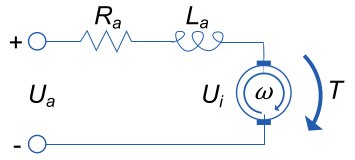
\includegraphics[width=0.32\columnwidth]{assets/dc-motor.png}
\end{wrapfigure}
(Kirchoff) $U_a = L_a \dot{I_a} + R_a I_a + U_i$

(Torque, Lorenz Force) $T = k_T I_a$

(Induced V, Faraday) $U_i = k_i \omega$

(Mech. pow. eq. el. pow)\\
$U_i I_a = k_i \omega I_a = T_\omega = k_T I_a \omega \Rightarrow k_i = k_T =: k$
